\chapter{Mô hình hóa cấu trúc}

\section{Phương pháp xác định lớp}

Áp dụng kỹ thuật \textbf{phân tích danh từ} (noun analysis) trên bốn biểu mẫu và mô tả quy trình (Chương 2), nhóm rút ra các danh từ ứng viên rồi loại bỏ: (i) danh từ trùng lặp/đồng nghĩa, (ii) thuộc tính thực chất là thuộc tính, (iii) danh từ ngoài phạm vi. Kết quả: 15 lớp doanh nghiệp.

\begin{table}[h]
\centering
\caption{Danh sách lớp doanh nghiệp và trách nhiệm}
\label{tab:classes}
\begin{tabular}{P{3.4cm}P{12cm}}
\toprule
\textbf{Lớp} & \textbf{Trách nhiệm} \\
\midrule
NguoiDung & Tài khoản người dùng: đăng nhập, thông tin cá nhân, thuộc một vai trò và (tùy chọn) một đơn vị \\
VaiTro & Định nghĩa vai trò phân quyền: DON\_VI, VAN\_PHONG\_CUC, LANH\_DAO\_CUC, QMS, NHA\_THAU \\
DonVi & Đơn vị/phòng thuộc Cục sử dụng thiết bị \\
TrangThietBi & Thiết bị: thuộc tính đúng BM/01 (mã số, tên, nước sản xuất, ngày nhận, đơn vị); trạng thái vòng đời; kiểm tra nhắc bảo dưỡng \\
HoSoThietBi & Một bản ghi lịch sử của thiết bị — đúng bảng BM/02 (ngày thực hiện, nội dung, người thực hiện); chỉ thêm, không sửa/xóa \\
KeHoachBaoDuong & Kế hoạch năm (BM/03 — header): năm, trạng thái phê duyệt, người duyệt \\
ChiTietKeHoach & Hạng mục kế hoạch (BM/03 — dòng): nội dung, đơn vị thực hiện (nội bộ/bên ngoài), tháng dự kiến, ghi chú; trạng thái tiến độ \\
SuCo & Sự cố: mã, mô tả, mức độ, phân loại xử lý, trạng thái theo vòng đời xử lý \\
PhuongAnSuaChua & Phương án sửa chữa/thuê ngoài: nội dung, chi phí dự kiến, trạng thái phê duyệt \\
NhaThau & Nhà cung cấp dịch vụ bảo dưỡng/sửa chữa ngoài (mở rộng) \\
BienBanNghiemThu & Biên bản nghiệm thu (BM/04): nội dung đã thực hiện, tình trạng sau thực hiện, ngày lập, số bản (02) \\
DaiDien & Người đại diện hai bên trong biên bản: bên (A/B), họ tên, đơn vị, đã ký \\
TaiLieuDinhKem & File đính kèm đa hình: gắn vào thiết bị/sự cố/nghiệm thu/kế hoạch \\
ThongBao & Thông báo trong hệ thống (nhắc lịch, phê duyệt, sự cố) \\
NhatKyHeThong & Audit trail append-only: hành động, đối tượng, dữ liệu cũ/mới (ISO 9001) \\
\bottomrule
\end{tabular}
\end{table}

\section{Thẻ CRC}

\begin{table}[h]
\centering
\begin{tabular}{|P{5.2cm}|P{5.2cm}|}
\hline
\multicolumn{2}{|l|}{\textbf{Lớp: TrangThietBi}} \\
\hline
\textbf{Trách nhiệm (Responsibilities)} & \textbf{Cộng tác viên (Collaborators)} \\
\hline
Giữ thông tin nhận dạng thiết bị (BM/01) \newline Quản lý trạng thái vòng đời \newline Cung cấp lịch sử hồ sơ \newline Kiểm tra hạng mục bảo dưỡng đến hạn & HoSoThietBi (tạo bản ghi) \newline DonVi (thuộc đơn vị) \newline SuCo (gắn sự cố) \newline ChiTietKeHoach (gắn kế hoạch) \\
\hline
\end{tabular}
\end{table}

\begin{table}[h]
\centering
\begin{tabular}{|P{5.2cm}|P{5.2cm}|}
\hline
\multicolumn{2}{|l|}{\textbf{Lớp: SuCo}} \\
\hline
\textbf{Trách nhiệm} & \textbf{Cộng tác viên} \\
\hline
Tiếp nhận báo sự cố \newline Chuyển trạng thái xử lý \newline Định tuyến: tự khắc phục / lập phương án \newline Đóng sự cố sau nghiệm thu & TrangThietBi (thiết bị hỏng) \newline NguoiDung (người báo, người xem xét) \newline PhuongAnSuaChua (tạo khi thuê ngoài) \newline BienBanNghiemThu (đóng khi đủ chữ ký) \\
\hline
\end{tabular}
\end{table}

\begin{table}[h]
\centering
\begin{tabular}{|P{5.2cm}|P{5.2cm}|}
\hline
\multicolumn{2}{|l|}{\textbf{Lớp: BienBanNghiemThu}} \\
\hline
\textbf{Trách nhiệm} & \textbf{Cộng tác viên} \\
\hline
Ghi nhận nội dung đã thực hiện và tình trạng sau thực hiện (BM/04) \newline Quản lý danh sách đại diện hai bên \newline Ghi hồ sơ thiết bị khi đủ chữ ký & DaiDien (hợp thành 2--4) \newline PhuongAnSuaChua (nguồn nghiệm thu) \newline HoSoThietBi (tự tạo bản ghi) \newline SuCo (đóng sự cố) \\
\hline
\end{tabular}
\end{table}

\section{Sơ đồ lớp}

\begin{figure}[h]
\centering
\IfFileExists{figures/class.png}{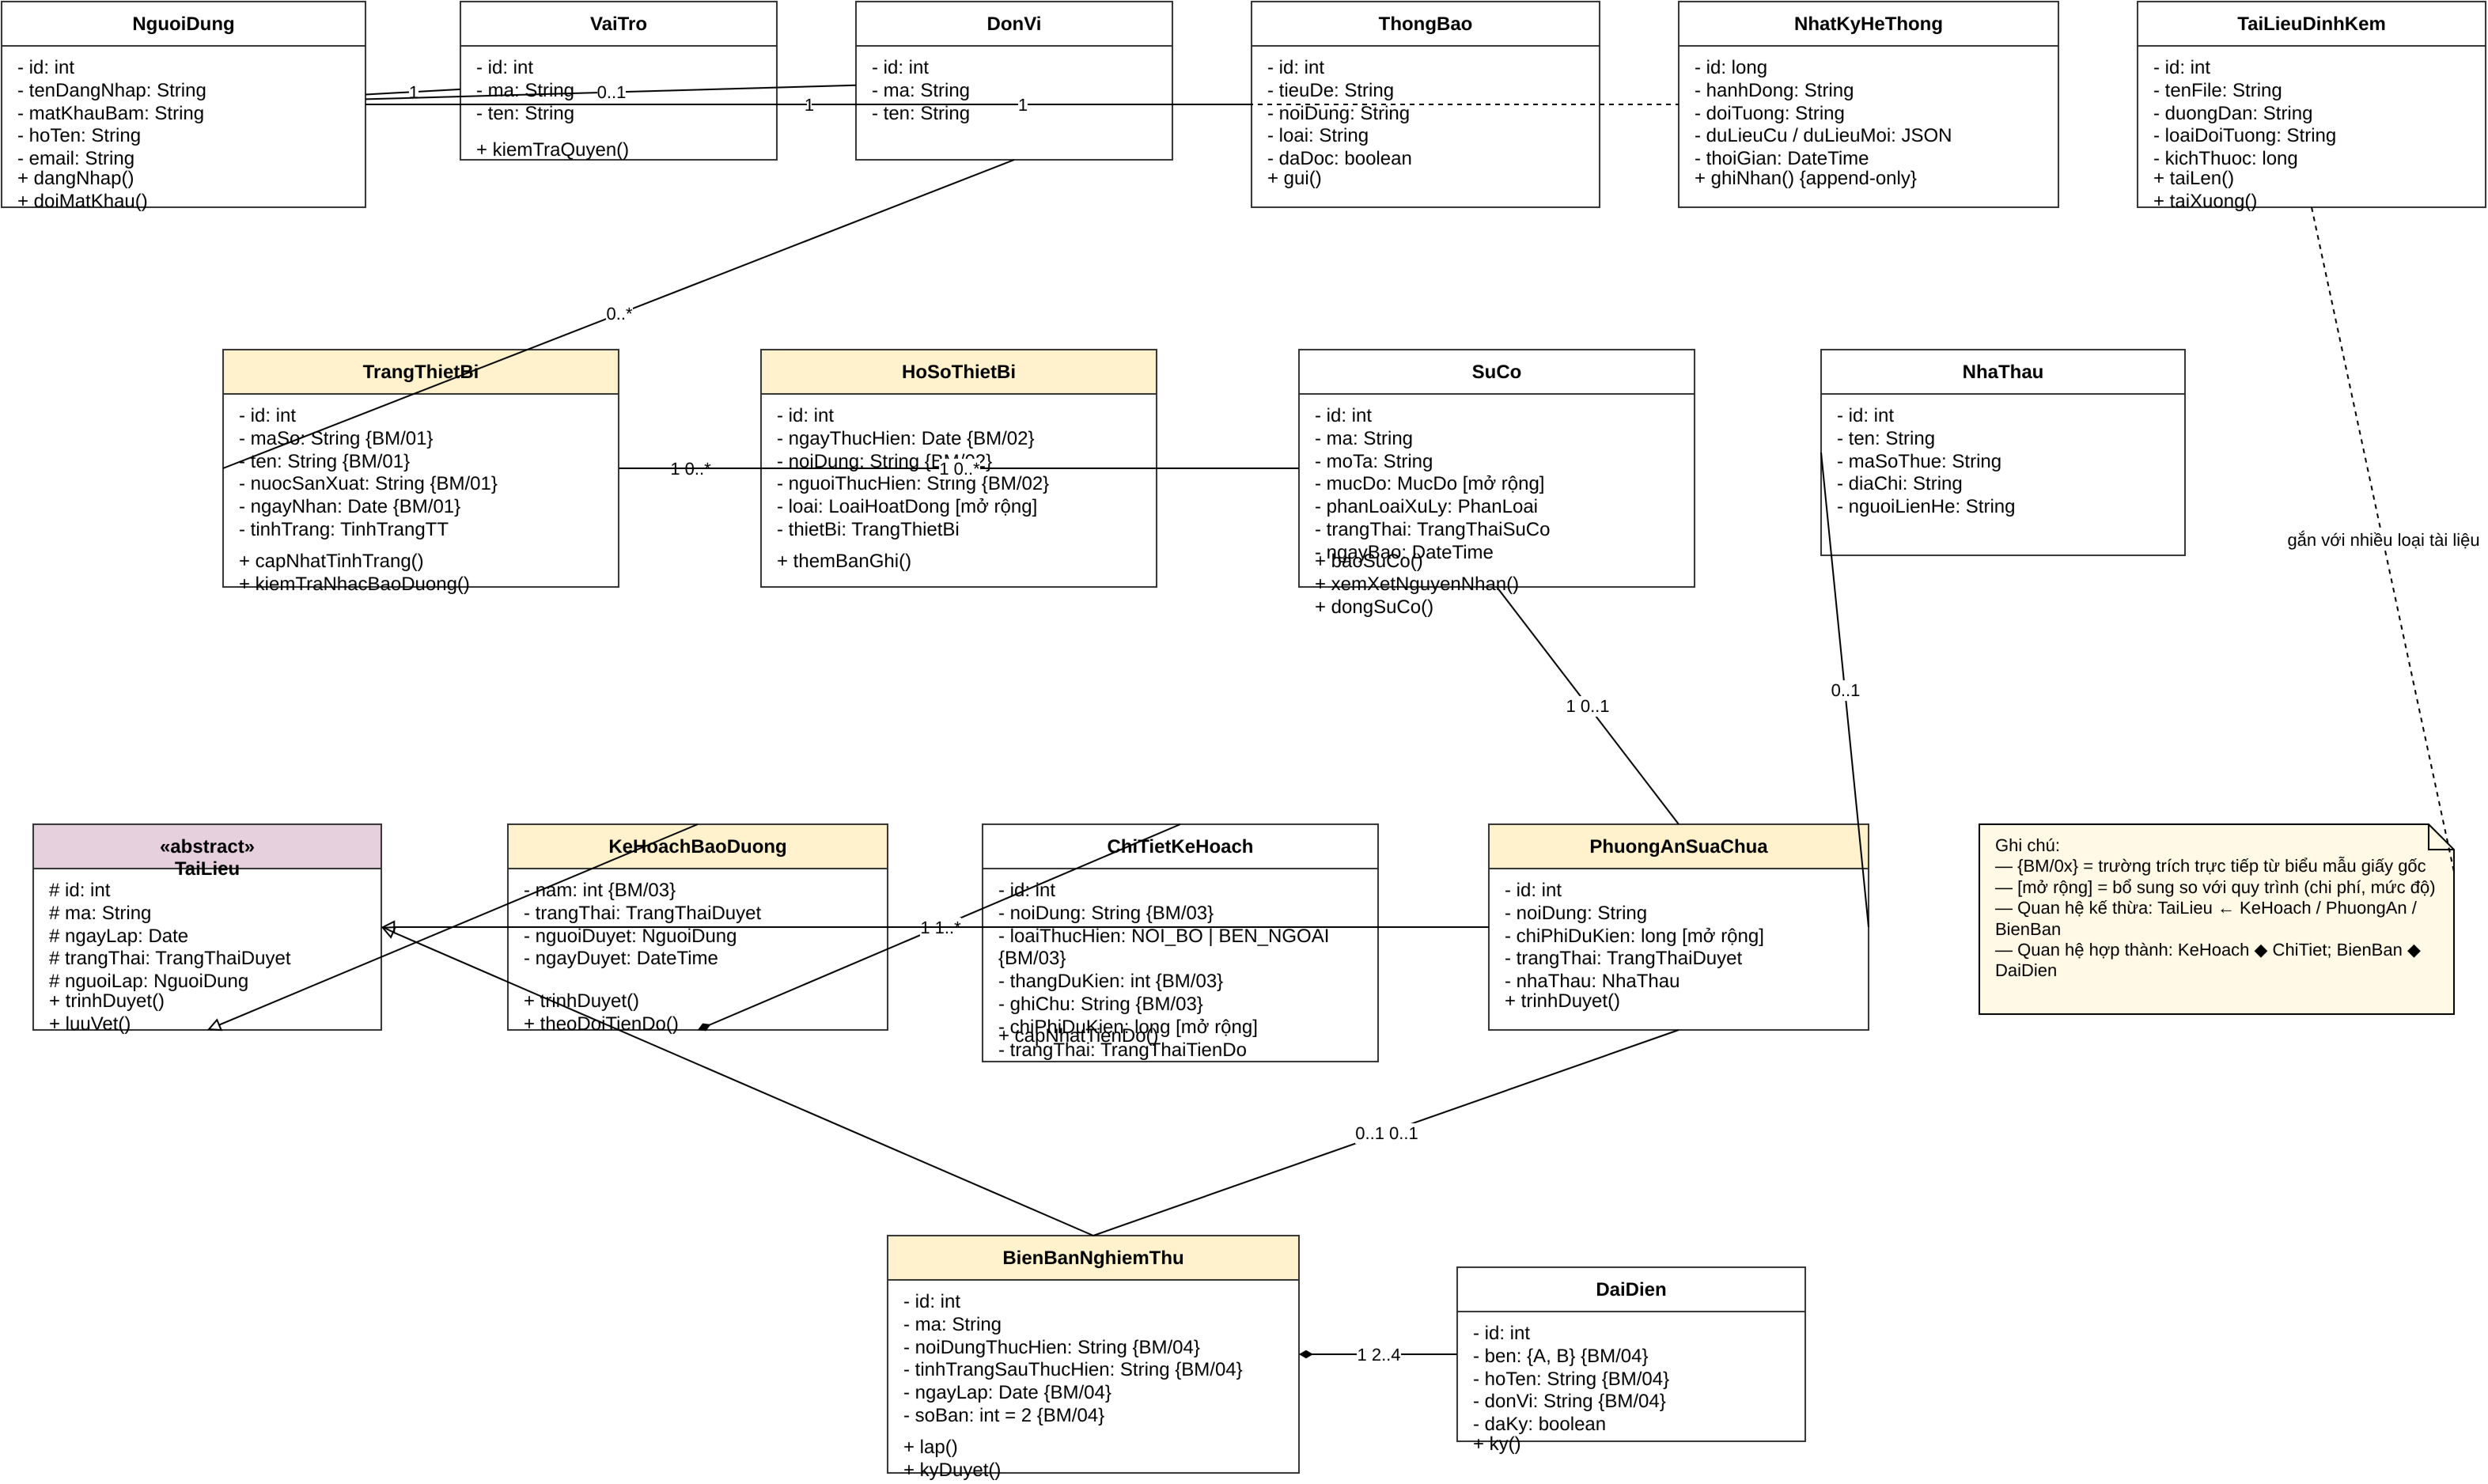
\includegraphics[width=\textwidth]{figures/class.png}}{\fbox{\parbox{0.9\textwidth}{\centering Sơ đồ lớp (file \texttt{docs/diagrams/03-class.drawio})}}}
\caption{Sơ đồ lớp của hệ thống}
\label{fig:class}
\end{figure}

\subsection{Các quan hệ chính}

\begin{itemize}
  \item \textbf{Kết tập/gắn kết một--nhiều:} TrangThietBi 1 --- 0..* HoSoThietBi; TrangThietBi 1 --- 0..* SuCo; SuCo 1 --- 0..1 PhuongAnSuaChua; PhuongAnSuaChua 0..1 --- 0..1 BienBanNghiemThu; ChiTietKeHoach * --- 1 TrangThietBi.
  \item \textbf{Hợp thành (composition):}
  \begin{itemize}
    \item \emph{KeHoachBaoDuong $\blacklozenge$--- 1..* ChiTietKeHoach}: hạng mục không tồn tại độc lập ngoài kế hoạch; xóa kế hoạch thì xóa hạng mục.
    \item \emph{BienBanNghiemThu $\blacklozenge$--- 2..4 DaiDien}: đại diện là cấu phần bắt buộc của biên bản (Bên A + Bên B, mỗi bên 1--2 người), đúng cấu trúc BM/04.
  \end{itemize}
  \item \textbf{Kế thừa (generalization):} lớp trừu tượng \emph{TaiLieu} (mã, ngày lập, trạng thái phê duyệt, người lập; hành vi \texttt{trinhDuyet()}, \texttt{luuVet()}) là lớp cha của \emph{KeHoachBaoDuong}, \emph{PhuongAnSuaChua}, \emph{BienBanNghiemThu} — ba loại ``tài liệu'' đều đi qua vòng đời trình duyệt và cần lưu vết.
  \item \textbf{Phân quyền:} NguoiDung * --- 1 VaiTro; NguoiDung * --- 0..1 DonVi.
  \item Trong sơ đồ, trường mang nhãn \{BM/0x\} trích trực tiếp từ biểu mẫu giấy; nhãn [mở rộng] là bổ sung đề xuất (chi phí, mức độ ưu tiên) — tách bạch với nguyên bản.
\end{itemize}

\subsection{Ánh xạ lớp $\rightarrow$ bảng dữ liệu}

Sơ đồ lớp được ánh xạ 1--1 sang lược đồ quan hệ PostgreSQL (chi tiết đầy đủ ở Chương 6): mỗi lớp một bảng; quan hệ nhiều--một qua khóa ngoại; hợp thành qua ràng buộc \texttt{ON DELETE CASCADE}; kế thừa TaiLieu được ``phẳng hóa'' (các thuộc tính chung lặp lại trong từng bảng con) vì số lượng lớp con ít và giúp truy vấn đơn giản — quyết định được cân nhắc trong thiết kế.
